% This is "aamas2012 .tex" August 2012 
% This file should be compiled with "aamas2012 .cls" 
% This example file demonstrates the use of the 'aamas2012 .cls'
% LaTeX2e document class file. It is for those submitting
% articles to AAMAS 2012  conference. This file is based on
% the sig-alternate.tex example file.
% The 'sig-alternate.cls' file of ACM will produce a similar-looking,
% albeit, 'tighter' paper resulting in, invariably, fewer pages.
% than the original style ACM style.
%
% ----------------------------------------------------------------------------------------------------------------
% This .tex file (and associated .cls ) produces:
%       1) The Permission Statement
%       2) The Conference (location) Info information
%       3) The Copyright Line with AAMAS data
%       4) NO page numbers
%
% as against the acm_proc_article-sp.cls file which
% DOES NOT produce 1) thru' 3) above.
%
% Using 'aamas2012 .cls' you don't have control
% from within the source .tex file, over both the CopyrightYear
% (defaulted to 200X) and the IFAAMAS Copyright Data
% (defaulted to X-XXXXX-XX-X/XX/XX).
% These information will be overwritten by fixed AAMAS 2012  information
% in the style files - it is NOT as you are used with ACM style files.
%
% ---------------------------------------------------------------------------------------------------------------
% This .tex source is an example which *does* use
% the .bib file (from which the .bbl file % is produced).
% REMEMBER HOWEVER: After having produced the .bbl file,
% and prior to final submission, you *NEED* to 'insert'
% your .bbl file into your source .tex file so as to provide
% ONE 'self-contained' source file.
%

% This is the document class for full camera ready papers and extended abstracts repsectively 

\documentclass{llncs}
\usepackage{amsfonts} % if you want blackboard bold symbols e.g. for real numbers
\usepackage{graphicx} % if you want to include jpeg or pdf pictures
\usepackage{lmodern}
\usepackage{amsmath}
\usepackage{amssymb}
\usepackage{algorithmic}
\usepackage{algorithm}


\usepackage{pgfplots}
\usepackage{filecontents}
\usepackage{tikz}
\usepackage{tree-dvips}
\usetikzlibrary{positioning}
\pgfplotsset{compat=newest}



% if you are using PDF LaTex and you cannot find a way for producing
% letter, the following explicit settings may help
 
\pdfpagewidth=8.5truein
\pdfpageheight=11truein

\begin{document}

% In the original styles from ACM, you would have needed to
% add meta-info here. This is not necessary for AAMAS 2012  as
% the complete copyright information is generated by the cls-files.


\title{Solving the Coalition Structure Generation Problem on a GPU}

% AUTHORS


% For initial submission, do not give author names, but the
% tracking number, instead, as the review process is blind.

% You need the command \numberofauthors to handle the 'placement
% and alignment' of the authors beneath the title.
%
% For aesthetic reasons, we recommend 'three authors at a time'
% i.e. three 'name/affiliation blocks' be placed beneath the title.
%
% NOTE: You are NOT restricted in how many 'rows' of
% "name/affiliations" may appear. We just ask that you restrict
% the number of 'columns' to three.
%
% Because of the available 'opening page real-estate'
% we ask you to refrain from putting more than six authors
% (two rows with three columns) beneath the article title.
% More than six makes the first-page appear very cluttered indeed.
%
% Use the \alignauthor commands to handle the names
% and affiliations for an 'aesthetic maximum' of six authors.
% Add names, affiliations, addresses for
% the seventh etc. author(s) as the argument for the
% \additionalauthors command.
% These 'additional authors' will be output/set for you
% without further effort on your part as the last section in
% the body of your article BEFORE References or any Appendices.

%\numberofauthors{8} %  in this sample file, there are a *total*
% of EIGHT authors. SIX appear on the 'first-page' (for formatting
% reasons) and the remaining two appear in the \additionalauthors section.
%


% You can go ahead and credit any number of authors here,
% e.g. one 'row of three' or two rows (consisting of one row of three
% and a second row of one, two or three).
%
% The command \alignauthor (no curly braces needed) should
% precede each author name, affiliation/snail-mail address and
% e-mail address. Additionally, tag each line of
% affiliation/address with \affaddr, and tag the
% e-mail address with \email.
% 1st. author
\author{Kim Svensson,\inst{1} Sarvapali D. Ramchurn,\inst{1} Francisco Cruz,\inst{2} Juan-Antonio Rodriguez-Aguilar,\inst{2} Jesus Cerquides\inst{2}}
\institute{Electronics and Computer Science, University of Southampton, SO17 1BJ, UK
\email{\tt\{ks6g10,sdr\}@ecs.soton.ac.uk} 
\and
IIIA, CSIC, Spain
 \email{\tt\{tito,jar,jesus\}@iiia.csic.es}
}

\maketitle

\begin{abstract}
We develop the first parallel algorithm for Coalition Structure Generation (CSG), which is central to many multi-agent systems applications. Our approach involves distributing the key steps of a dynamic programming approach to CSG across computational nodes on a Graphics Processing Unit (GPU) such that each of the thousands of threads of computation can be used to perform small computations that speed up the overall process. In so doing, we solve important challenges that arise in solving combinatorial optimisation problems on GPUs such as the efficient allocation of memory and computational threads to every step of the algorithm. In our empirical evaluations on a standard GPU,  our results show an improvement of orders of magnitude over current dynamic programming approaches with an ever increasing divergence between the CPU and GPU-based algorithms in terms of growth. Thus, our algorithm is able to solve the CSG problem for 29 agents in one hour and thirty minutes as opposed to three days for the current state of the art dynamic programming algorithms.
\end{abstract}

% Note that the category section should be completed after reference to the ACM Computing Classification Scheme available at
% http://www.acm.org/about/class/1998/.

%\category{H.4}{Information Systems Applications}{Miscellaneous}

%A category including the fourth, optional field follows...
%\category{D.2.8}{Software Engineering}{Metrics}[complexity measures, performance measures]

%General terms should be selected from the following 16 terms: Algorithms, Management, Measurement, Documentation, Performance, Design, Economics, Reliability, Experimentation, Security, Human Factors, Standardization, Languages, Theory, Legal Aspects, Verification.

%\terms{Delphi theory}

%Keywords are your own choice of terms you would like the paper to be indexed by.

%\keywords{AAMAS proceedings, \LaTeX, text tagging}

\section{Introduction}
\noindent Coalition formation is one of the key coordination mechanisms in
multi-agent systems. It involves the coming together of a number of  agents to
achieve some individual or group objective.  An important step in the 
 coalition formation process involves partitioning the set of agents into coalitions that, on aggregate (as a coalition structure), maximise the efficiency in the system. This problem is termed the 
\emph{Coalition Structure Generation} problem (CSG)
~\cite{DBLP:journals/ai/SandholmLAST99}.   The  CSG problem is a hard combinatorial optimisation problem and scales in $\omega(n^n)$ \cite{DBLP:journals/ai/SandholmLAST99}. To date, many algorithms have been designed to solve the CSG. These range from branch-and-bound approaches such as \cite{rahwan2009anytime}, to dynamic programming approaches such as
\cite{DBLP:conf/atal/RahwanJ08,rahwan:jennings:2008b}. The latter are particularly attractive given their lower complexity, but most of these algorithms scale to around 30 agents given the exponential growth in computation involved. We also note that these algorithms were mainly designed for single-threaded architectures, and even if distributed variants exist \cite{michalak2010distributed}, these require storing the input data redundantly across multiple computers and sharing information over network links that may be liable to delays and losses. 

In contrast, in the last few years, a surge in the development of frameworks for parallel programming on a single machine has been noted with the development of general-purpose Graphics Processing Units (GPUs). Indeed, these processors, originally developed for only processing high end graphics, can now be programmed to perform simple mathematical operations that, when performed in thousands in parallel, can significantly outperform single-threaded machines with higher frequencies and memory speeds. There are multiple challenges, however, that need to be overcome before complex algorithms as for CSG can be implemented onto the GPU (we elaborate on these in Section \ref{sec:gpu-csg}) including the need to limit random memory access,  the limits on the number of threads that can be launched to share the same memory blocks, and the need to avoid loading data frequently from main memory. 

Against this background, in this paper, we present a parallel algorithm for CSG for highly multi-threaded GPUs that meets the challenges above and outperforms the best algorithms for CSG. Our algorithm, GPU-CSG, parallelises the computation of individual steps of a dynamic program to solve the CSG. It does so by partitioning the computation across thousands of threads where each solves a small sub-problem of the larger optimisation problem. The solution to each sub-problem is then used to find the best partition of agents. In more detail, this paper advances the state of the art in the following ways. First, we develop the first parallel  algorithm for CSG that avoids redundant memory storage and inter-processor communication. Second, we prove that GPU-CSG is correct and complete and demonstrate through empirical evaluation that its growth rate is significantly lower than that of the dynamic programming approach it builds upon. Third, we empirically show that GPU-CSG outperforms the state of the art by orders of magnitude, solving the CSG problem for 29 agents in less than 1.5 hours as opposed to 83 hours for the CPU-based algorithm.

The rest of this paper is structured as follows. Section 2 presents the
background to this work and discusses related work, as well introduces the
the GPU architecture and details the DP algorithm. Section 3 and 4 then details the GPU-CSG which is built upon the DP algorithm,
while Section 5 concludes.

\section{Background}
Solving data-independent and parallel problems will always have a benefit when run on a GPU, 
whether it is computing on MRI scans, which gave a significantly large speedup factor of 431 using the GPU, or generating hashes and getting a comparably modest speedup of times 11~\cite{ryoo2008optimization}.  This is particularly the case whenever the algorithm has data-independent sub-routines which may be run concurrently. If so the GPU will most likely perform better. Combining the GPU together with dynamic programming has been used before to solve similar combinatorial optimisation problems.  Boyer, et al. successfully implemented and solved the knapsack problem with a factor speedup of 26~\cite{boyer2012solving}.  They also introduced ways to reduce memory usage and thus enable computation of much larger data sets, as well as reduce the  bandwidth utilised. In so doing, they also reduce computation time by being able to fetch more data points at an faster rate. Thus, they fully exploit the key features of GPU programming whereby, with limited amount of memory available on a GPU,  they are able to maximise the effective bandwidth of the algorithm.

Now, turning to the CSG problem, in terms of parallel programming approaches, we note the work of Michalak et. al. that uses a distributed variant of the anytime IP algorithm called D-IP to solve the Coalition Structure Generation~\cite{michalak2010distributed}. They use 14 dual-core workstations to distribute the workload to speed up their run-time. Their algorithm  shows it is possible to distribute the solutions for the CSG problem and that there may be significant from distributing computation (taking only 11\% to 4\% of the time, compared to the centrilised and serialised IP). However, while their algorithm use traditional programming strategies effective on powerful single-threaded systems, it does require data to be shared between computational nodes over potentially slow Ethernet links and also sharing redundant copies of the input across each. Finally, their algorithm also suffers from the same weaknesses as IP, that is, no deterministic completion time (in the worst case ($O(n^n))$ as it is dependent on the coalition value function. In contrast, GPU-CSG has a deterministic completion time ($O(3^n)$) and relies on much faster GPU memory access.

In what follows, we first describe the CUDA architecture (the GPU architecture provided by Nevada) to clarify what are the key features and issues of using GPUs to solve large combinatorial problems. We then describe the DP algorithm and the data structures we use to implement it on the CUDA architecture.

\subsection{The CUDA Architecture} \label{Cuda} %done
Graphics Processing Units (GPUs) from NVIDIA and AMD are highly multi-threaded, many-core architectures primarily aimed at highly parallel image processing and rendering. In recent years, however, there has been a move to use these to support more general-purpose computing through the OpenCL and NVIDIA CUDA framework. This was achieved by devoting a larger amount of transistors towards many computational units rather than data caching and advanced  flow control more often seen in CPU architectures. NVIDIA describes their general-purpose GPU CUDA architecture as a Single Instruction Multiple Threads (SIMT) architecture, meaning groups of multiple threads execute the same instructions concurrently and is proportional to SIMD architectures. 
This enables their GPUs to be highly advantageous when performing data-independent and non-divergent tasks. To understand this further the grouping of the threads need to be explained and is outlined in figure \ref{fig:reduction}.
\begin{figure*}
\centering
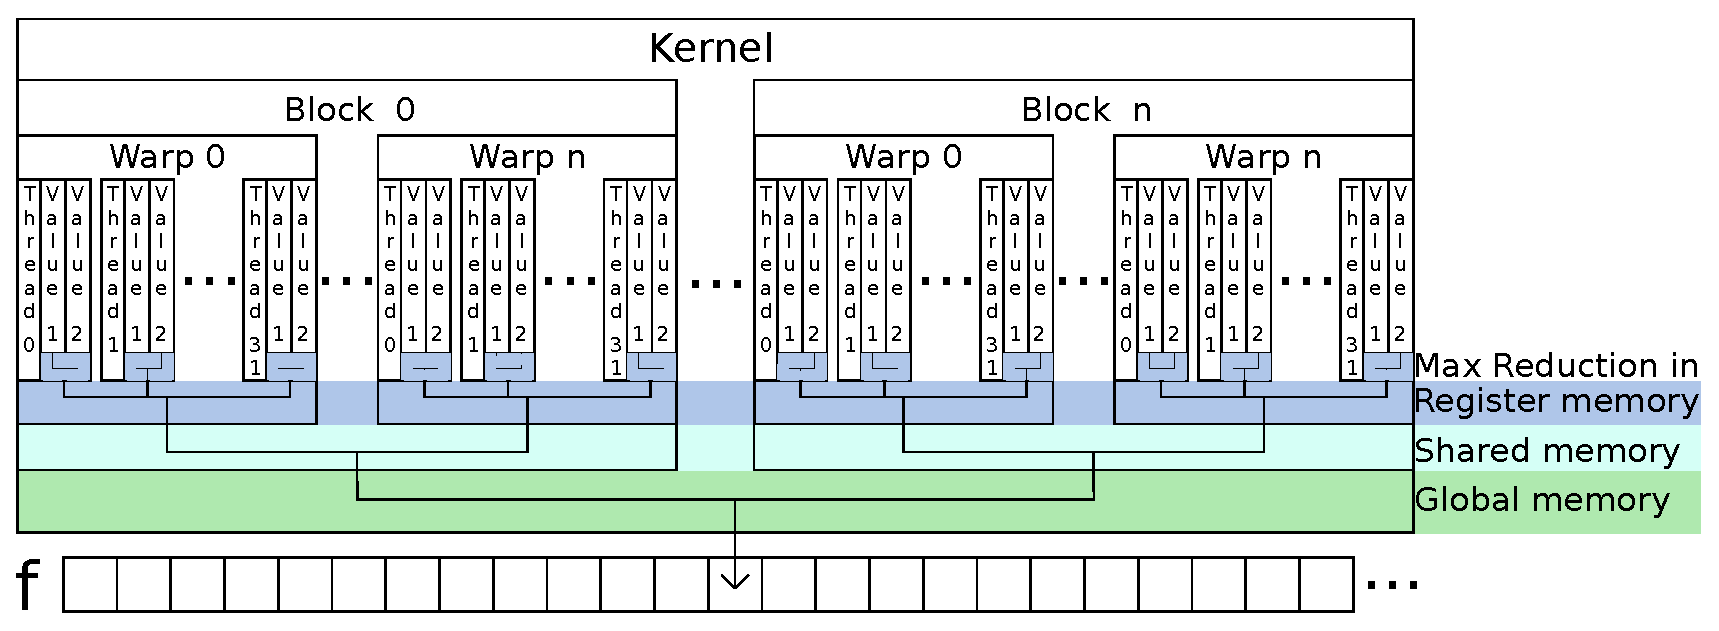
\includegraphics[width=\linewidth]{reduction}
\caption{Outline of reduction across thread, warp, block and kernel \label{fig:reduction}. The kernel is a function called by the CPU.}
\end{figure*}
The kernel is a device-specific CUDA function that is called by the sequential host code, which will request a specified number of blocks in a grid of blocks. Each block may to this date consist of up to 1024 threads depending on the compatibility of the card, with a maximum grid size of $2^{31}-1$ blocks subjected to compatibility. When run, the blocks will be distributed onto available multiprocessors, which then independently schedule the run-time of the block. Note that blocks may be executed concurrently or sequential depending on the current workload and the number of available multiprocessors. The block is split into smaller units of 32 threads called warps, all threads within the same warp are always scheduled the same instruction to be run and this is what embodies the SIMT \footnote{Single Instruction Multiple Threads (SIMT) architecture, All threads inside a warp execute the same instruction} paradigm.  Therefore, branching threads causing intra-warp divergence means a warp will have inactive threads not executing any instructions,  which may lead to poor efficiency with worst case of sequential performance. Further, warps are scheduled independently of each other meaning possible concurrent execution of warps.

The threads communicate with each other through writes to various types of memory outlined in table \ref{mem}. There are three types of thread writable memory in the architecture; registers and local memory are each threads coupled memory, which is not volatile and may be shared with other threads inside the same warp as described in Section \ref{reduction}.  Shared memory is as its name tells is shared between all threads within the same block, as it may be written to by any thread within the block it should be treated as volatile, thus synchronization inside the block have to be consider whilst dealing with shared memory. Finally, global memory is the only persistent memory, which will persist between each kernel call, it may be manipulated by the host, but also by any thread, and is the only means of communication in between kernels, blocks, and the host.

Now, an important element of GPU programming is to manage the access to global memory effectively as it is very slow compared to memory access of the on-chip memory on the GPU. In more detail, each load request from memory will fetch in cache-lines of size $32*wordsize$, meaning cache-lines of 32, 64, and 128 bytes each when pulling the primitives char, short and int respectively. This is because, as mentioned earlier, all 32 threads within the same warp issue the same instruction.  Thus each warp fetches 32 entities of a specific word type, if the memory reads within a warp is not coalesced (grouped within the same cache-line) within consecutive words, the effective bandwidth will drop immediately. Table \ref{mem} summarises the key features of GPU memory access speeds and shows why it is important to avoid loading data from the global memory.

\begin{table}
\centering
\caption{Memory scope, lifetime, and speed \label{mem}}
\begin{tabular}{|l|l|l|l|} \hline
Type&Scope&Lifetime&Relative Speed \\ \hline
Register&Thread \& Warp&Thread&Fastest\\
Shared&Block&Block&Fast\\
Global&Kernel \& Host&Program&Slow\\
\hline\end{tabular}
\end{table}
In the next subsection, we describe the DP algorithm, which we build upon.
\subsection{The {DP} Algorithm} 
%done
The DP algorithm \cite{DPalgorithm} was originally designed to solve the winner determination problem for combinatorial auctions. However, in recent years, it has been applied as the de facto  algorithm (complete and with the lowest worst case complexity) to solve the CSG problem and variants of it have improved and adapted it to different settings \cite{DBLP:conf/atal/RahwanJ08,DBLP:conf/aamas/VoiceRJ12}. However, the core of the algorithm is the same in all these variants and relies on dynamic programming. Hence, in this paper we use this as the basis for our GPU version as the dynamic programming approach has shown potential for parallelisation as evidenced by previous work (as for the Knapsack problem as mentioned earlier). 

To show how the algorithm works, we first formalise the CSG problem.  Let $A=\{1,\ldots,\vert A \vert \}$ be a set of agents. A subset $C \subseteq A$ is termed a coalition.  Then, a $CSG$ problem is completely defined by its characteristic function $v: 2^{A} \rightarrow \Re$ (with $v(\emptyset)=0$), which assigns a real value representing utility to every feasible coalition.  The CSG problem is to identify the exhaustive disjoint partition of the space of agents into coalitions (or, \emph{coalition structure})  $CS=\{C_1,\ldots,C_k\}$ so that the total sum of values, $\sum^k_{i=1} v(C_k)$,
is maximised.

Now, DP (see Algorithm  \ref{DP}) works by producing two output tables, $O$ and $f$, 
where each table has one entry per coalition structure. 
An entry in $f$ represents a value a certain coalition structure is given, 
while $O$ represent which splitting, if any, maximised the coalition structure for the entry in $f$ that it represents.
More elaborated, given all coalitions of agents $C\subseteq A$, for each coalition in $C$, evaluate all
pairwise disjoint subsets (here named splittings) on their pairwise collective sum against the coalitions
original value. Given one splitting is greater, update the value of the coalition $f(C) := f(C') + f(C\setminus C')$
and assign $O$ on $C$ to represent the new splitting, $O(C) := \{C',C\setminus C'\}$. These steps are first carried out on all coalition structures with two agents, continuing until $|A|$ agents.  This means, given a coalition structure $S$ with cardinality $|S| = n$, then all coalition structures
for the sizes $1,2,...,n-1$ have already been evaluated. The dynamic programming algorithm is entirely deterministic meaning that even if there was only one or two valuations, the algorithm will evaluate all splittings before it reaches a conclusion. However this algorithm does not work well with a large number of agents as it grows exponentially and has time and memory complexity $O(3^n)$. As described later in Section \ref{algorithm}, the part of the algorithm that is parallelized is the max function on line \ref{lst:line:a}, which handles the evaluation of all splittings of a given coalition structure.

\begin{algorithm}
\caption{Dynamic Programming algorithm \label{DP}}
INPUT: $v$: collection of the bids for all coalitions\\*
VARIABLES: $f$: collection holding the maximum value for all coalitions\\*
$O$: collection holding the most beneficial splitting for all coalitions.
\begin{algorithmic}[1]
\STATE\algorithmicfor\ all $x \in A$, \algorithmicdo  $f(\{x\}):= v(\{x\}),O\{x\}:= \{x\}$ \algorithmicendfor
\FOR{$i := 2$ to $n$}
\FOR{all $C \subseteq A: \vert C \vert == i$}
\STATE $f(C) := max\{f(C\backslash C')+f(C'):C'\subseteq C \wedge 1 \leq \vert C' \vert \leq \dfrac{\vert C \vert}{2}\}$ \label{lst:line:a}
\STATE\algorithmicif $f(C) \geq v(C)$ \algorithmicthen\ $O(C) := C^{*}$ \hfill Where $C^{*}$ maximizes right hand side of line~\ref{lst:line:a} \algorithmicendif
\STATE\algorithmicif $f(C) < v(C)$ \algorithmicthen\ $f(C) := v(C)\wedge O(C) := C$ \algorithmicendif
\ENDFOR
\ENDFOR
\STATE Set $CS^* := \{A\}$
\FOR{all $C \in CS^*$} \label{lst:line:redo}
\IF{$O(C) \neq C$}
\STATE Set $CS^* := (CS^*\setminus \{C\})\cup \{O(C),C\setminus O(C)\}$ 
\STATE Goto \ref{lst:line:redo} and start with a new $CS^*$
\ENDIF
\ENDFOR
\RETURN $CS^*$
\end{algorithmic}
\end{algorithm}

The table $O$ may be discarded and not calculated to reduce memory requirements by half removing instant access to the final splittings. These final splittings are easily retrieved as outlined in algorithm \ref{idpref}.  Essentially, all coalitions in $C \in CS^*$ whose value in $f$ is not equal to the initial value in $v$, find the first splitting that is equal to the value in $f$. The overhead of this is insignificant as it needs to evaluate at most $n -1$ coalitions compared to the exponential
number of evaluations carried out in the previous steps\cite{eps265062}.

\begin{algorithm}
\caption{Enumeration of the optimal splittings through re-evaluation of small amount of coalitions \label{idpref}}
INPUT: $v:$ array of the initial bids for all coalitions $C \subseteq A$. 
$f:$ the final evaluated values gathered from evaluating splittings.
\begin{algorithmic}[1]
\STATE Set $CS^* := \{A\}$
\FOR{all $C \in CS^*$} \label{lst:line:redo2}
\IF{$f(C) \neq v(C)$}
\STATE find first $C^*$ where $f(C) = f(C\backslash C^*)+f(C^*):C^*\subseteq C \wedge 1 \leq \vert C^* \vert \leq \dfrac{\vert C \vert}{2}$ \label{lst:line:aa}
\STATE Set $CS^* := (CS^*\setminus \{C\})\cup \{C^*,C\setminus C^*\}$
\STATE Goto \ref{lst:line:redo2} and start with a new $CS^*$
\ENDIF
\ENDFOR
\RETURN $CS^*$
\end{algorithmic}
\end{algorithm}
Having described the DP algorithm, we next elaborate on the data structure we use to extend DP into GPU-CSG and then go on to detail the algorithm.

\section{GPU-CSG} \label{sec:gpu-csg} %done
GPU-CSG parallelises the key steps of the DP algorithm. This is a non-trivial process (as we will see) as it requires us to be efficient in memory access and in sharing the computation among the threads on the GPU so that access to global memory is reduced while minimising the need for synchronising the threads. To this end, we first propose a memory efficient technique to store coalitions and their values in memory. This is important because (as discussed  in Section 2), the GPU typically have relatively smaller amounts of memory. Moreover, we discuss different ways to navigate through the search space of coalitions as DP requires splitting coalitions into their components to evaluate each sub-problem separately.
\subsection{The Data Structure}\label{sec:data}
How data is represented and structured is important, especially in bandwidth bound algorithms where the majority of time is spent fetching data from memory and the arithmetic overhead is low.
Selecting the right composition will reduce the memory requirements substantially. Given the two entities of data that are needed to be represented for each coalition structure, the coalition structure itself and its value in $f$, we propose data structures that aim to allow a large number of agents to be represented in spite of the exponential growth of the input (i.e., $2^n$).

In order to minimize memory usage we applied several techniques as follows. First, we represent each coalition as a fixed sized array of values, where each value represents a distinct agent. While this may seem intuitive at first, if the members are represented as bits set in a fixed sized integer, the memory
requirement will be reduced substantially as shown by previous studies~\cite{boyer2012solving}.
When solving the CSG problem with $n$ agents representing members as an array of values, there are \[\dbinom{n}{i}\] coalition structures of size $i$, where $i$ entries have to be stored per coalition structure.

The total number of values needed to store just to represent the coalition structures is therefore equal to:
\begin{displaymath}\sum_{i=i}^{n} \dbinom{n}{i}\times i\end{displaymath}

Given the same constraints, representing the coalition structure as an fixed sized integer, it is only 
needed to store one entry per coalition, which is all together \begin{math}2^n-1\end{math} data points.

To give an example, with four agents $A = {f_0,f_1,f_2,f_3}$, the coalition $C = {f_0,f_2,f_3}$ would be represented as $C = 1101$ in the binary system and $13$ in the decimal system. Therefore, if the coalition structure is represented as an integer it can implicitly be stored as an index to its coalition value, by enumerating it at run-time. That means the only memory constraint on the system is the storage for all coalition values.

Given that the index to the value of a coalition structure is as a binary representation, the distribution of, coalition structures 
that are lexicographically adjacent with the same cardinality will be evenly distributed over the fixed sized array.
This rise two constraints. First, the whole fixed sized array have to fit into the memory of the GPU, limiting the number of agents that can be represented. Second, fetching values will be in non-coalesced manner causing waste of bandwidth, which to some degree is resolved by detecting values that can be shared between coalition structures, as described in Section \ref{sectionsplit}.


Now, having defined coalitions as binary arrays, we next move on to explain how we create splittings of such coalitions efficiently for our algorithm to go through sub-solutions of the CSG problem.
\subsubsection{Coalition Structure Splittings}

% \begin{table}
% \centering
% \caption{Initialize shift on $C = \{f_0,f_2,f_3\}$\label{split}}
% \begin{tabular}{|l|r|r|} \hline
% Binary&$1_3 1_2 0_1 1_0$&\\ \hline
% Shift&\vline 0\vline 3\vline 2\vline 0\vline& Result \\ \hline
% Splitting 1 & $0001 : 1 << shift[0]$& $0001$ \\ 
% Splitting 2 & $0010 : 1 << shift[1]$&$ 0100$ \\
% Splitting 3 & $0011 : 1 << shift[0]$&\\ & $+ 1 << shift[1]$&$0101$ \\
% \hline\end{tabular}
% \end{table}

Splittings as mentioned are pairwise disjoint subsets of a coalition structure, 
given the coalition structure $C = \{f_3,f_2,f_0\}$ the splittings
are shown in table \ref{split}. In order to generate the splitting there are essentially three methods used:  $initShift$, $initialSplit$, and $nextSplit$. 

\begin{table}[htbp]
\centering
\caption{Splittings of $C = \{f_3,f_2,f_0\}$ Binary $C = 1101$ \label{split}}
\begin{tabular}{|l|c|c|c|} \hline
Set& $\{f_0\}$,$\{f_3,f_2\}$ &$\{f_2\},\{f_3,f_0\}$&$\{f_3\},\{f_2,f_0\}$ \\ 
system&&& \\ \hline	
Binary&0001\hfill 1100&0100\hfill 1001&1000\hfill 0101 \\
system&&& \\
\hline\end{tabular}
\end{table}

The function $initShift$, as detailed in Algorithm \ref{initshift} and partly illustrated in Figure \ref{fig:howitworks}, 
 is necessary to setup the environment for all calls to $initialSplit$.
 It takes as input the coalition structure that should be evaluated and the index $n$ which
represent the index for the coalition structure in the two dimensional array $shift$.
\begin{algorithm}
\caption{$initShift$ input $Coalition:C$ $Index:n$ \label{initshift}}
\begin{algorithmic}[1]
\STATE $t :=C$
\STATE $count := 0$
\WHILE{$t > 0$} { 
\STATE $index := FindFirstSet(t)$ \hfill Finds first bit set in t
\STATE $shift_{n,count} := index$ 
\STATE $nullBit(t,index)$ \hfill Sets one bit in t to zero
\STATE $count++$
}
\ENDWHILE
\RETURN shift
\end{algorithmic}
\end{algorithm}
The general idea is to put into the shared $shift$ array which members the coalition structure have in an ordered fashion. As illustrated in Figure \ref{fig:howitworks}, the coalition $C = \{f_3,f_2,f_0\}$ will have the values 0, 2 and 3 put in the array, these numbers represent which unique members it contains. It does so by using the bit operation $Find First Set$ which return the index of the first set bit, where the index represent which unique member in the coalition structure. It uses $Find First Set$ to find the first set bit in the coalition structure, and sets the bits index in the $shift$ array. Remove that member from the coalition structure by setting that bit to zero and scan for next set bit again, do so until all members have been identified and the coalition structure is empty. The two-dimensionality of the $shift$ array is to have one row in the array for each coalition structure that is being evaluated by the kernel. 
\begin{figure*}[htbp]
\centering
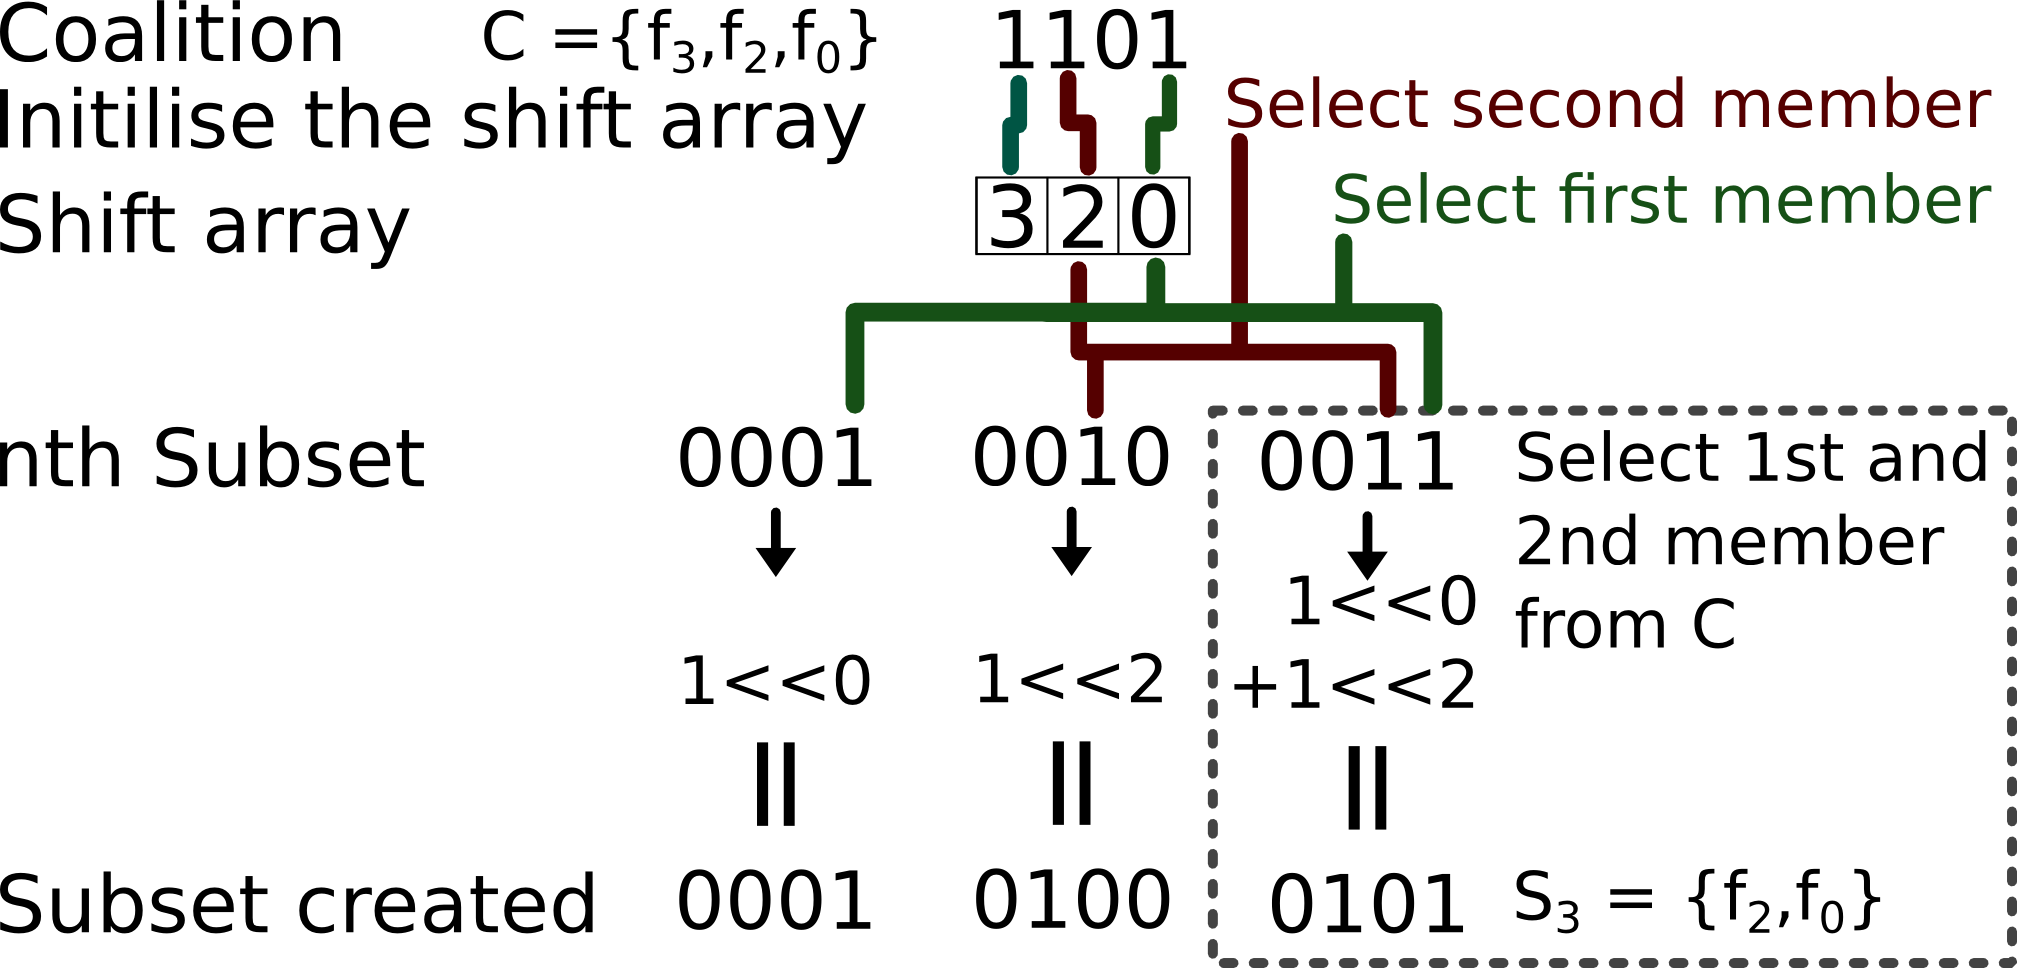
\includegraphics[width=0.7\linewidth]{test}
\caption{How initShift and initialSplit works\label{fig:howitworks}}
\end{figure*}

Further, using these values with the function $initialSplit$ described in Algorithm \ref{alg:initalsplit} to generate an initial splitting works as follows: Given the index $n$ as input that is an ascending integer value, which represent the $nth$ subset we want to create, and $C^*$ which represent the row in $shift$ for coalition structure $C$. The idea is to map the  bits set in $n$ to bits in the coalition structure $C$, effectively transforming members of $n$ to members in $C$. It does so by using $Find First Set$ to find the indexes of set bits in $n$, where the index will eventually represent the $n$th ordered member of coalition structure $C$. First, take the indexes of bits set in $n$ and use them to reference a column in row $C^*$ in the shift array, this will yield one member value $v$ from coalition structure $C$. To add that member to the subset to be created, take a single bit and binary left shift it $v$ places, and add it to the subset. Remove the set bit in $n$ and continue with previous operations until $n$ is empty. 

To illustrate as shown in Figure \ref{fig:howitworks}, the third subset represented as the binary value of $0011$, have its bits set in the indexes zero and one. In the shift array for coalition structure $C$, the indexes zero and one represent the first and secondly ordered members, which is agents $f_0$ and $f_2$ with values $v$ of 0 and 2. To form the subset, as described earlier, add together a single bit left shifted 0 places with a single bit left shifted 2 places. This will finally yield the subset $0101$ which have the members $f_0$ and $f_2$ in it. Then to generate the next splitting, a call to $nextSplit$ in Algorithm \ref{alg:nextsplit} is needed that works through a recurrence relation to generate the next splitting.

\begin{algorithm}
\caption{ nextSplit input $Coalition:C$ $Splitting:S$\label{alg:nextsplit}}
\begin{algorithmic}[1]
\STATE $C' := twosComplement(C)$
\STATE $S' := bitwiseAND((C'+S),C)$
\RETURN $S'$
\end{algorithmic}
\end{algorithm}

\begin{algorithm}
\caption{initialSplit input $index:n$ $index:C^*$\label{alg:initalsplit}}
\begin{algorithmic}[1]
\STATE $t := n$
\STATE $S := 0$
\WHILE{$t > 0$} { 
\STATE $index := FindFirstSet(t)$ \hfill Finds the first set bit in t
\STATE $S := S + leftShift(1,shift_{C^*,index})$ \hfill Shifts 1 left with the value in shift and adds
\STATE $nullBit(t,index)$ \hfill Sets the bit of t to 0
}
\ENDWHILE
\RETURN $S$
\end{algorithmic}
\end{algorithm}

\subsubsection{Collisions between Splittings of Coalitions} \label{sectionsplit}
Given that each thread evaluates several splittings over numerous coalition structures in parallel, 
it is bound that splittings on two coalitions that overlap will have splittings that collide.
A collision means that splittings of coalition contain at least one identical subset shared between them.
\begin{displaymath}\forall S\subset C \wedge S' \subset C' : C \cap C' \neq \emptyset \Rightarrow \exists S \wedge S' : S = S'\end{displaymath}
For all splittings of $C$ and $C'$ where the coalitions intersect, there exist at least one subset of a splitting shared between them.

The number of splittings that collide is dependent on how many common members the coalitions have in common.
\begin{displaymath}2^{n}-1:C\neq C'\wedge |C \cap C'| = n \wedge n > 1 \end{displaymath}
Specifically, the number of splittings in common is how many splittings
can be done on all the members of the intersection. Normally, each splitting would be fetched from global memory resulting in it being fetched several times, if it have not been evicted from the cache-memory.

For example, given two coalition structures $C_1 =\{f_0,f_1,f_2\}$ and $C_2 =\{f_0,f_1,f_3\}$ that intersect on $f_0$ and $f_1$, all splittings value where one subset only contain one or both members may be shared in-between them. I.e. the values for $S_1 = \{f_0\}$, $S_2 = \{f_1\}$, and $S_3 = \{f_0,f_1\}$ are interchangeable.

\begin{algorithm}[htbp]
\caption{Fetch using Collision detection \label{collision}}
Input:
Index:$\psi$ \hfill Which nth splitting should be generated
Index:$z$ \hfill The index in $\upsilon$ for the coalition structure that is evaluated 

Variables:Value $\alpha $: \hfill Holds temporary values

\begin{algorithmic}[1]
    \STATE $C_{0} := initialSplit(\psi,CS_0)$ \label{lst:line:startcol} \hfill Gets the splitting on $CS_0$ with index $\psi$
    \STATE $C_{1} := initialSplit(\psi,CS_1)$ \hfill Gets the splitting on $CS_1$ with index $\psi$
    \STATE $\upsilon_{0,z} := f(C_{0})$ \label{lst:line:fetch} \hfill Fetch the first value
    
    \IF{$C_{1} = C_{0}$} \label{lst:line:firstif} 
      \STATE $\upsilon_{0,z+1} := \upsilon_{0,z}$ \hfill Sets the other splittings value as its own
      \ELSE
      \STATE $\upsilon_{0,z+1} := f(C_{1})$ \hfill Else fetches its own value
     \ENDIF \label{lst:line:firstifend}
    \STATE $C_{0} := CS_0\backslash C_{0}$ \label{lst:line:startend} \hfill Get the other subset of the pairwise disjoint subset
    \STATE $\alpha := f(C_{0})$ \hfill Fetch the second value to a temporary variable
    \STATE $\upsilon_{0,z} := \upsilon_{0,z}  + \alpha$ \label{lst:line:endend} \hfill Add it
    \STATE $C_{1} := CS_1\backslash C_{1}$ \hfill Get the other subset of the pairwise disjoint subset
    \IF{$C_{1} = C_{0}$}
      \STATE $\upsilon_{0,z+1} := \upsilon_{0,z+1}  + \alpha$ \hfill Add the other splittings value to its own
    \ELSE
      \STATE $\upsilon_{0,z+1} := \upsilon_{0,z+1} + f(C_{1})$ \hfill Else add its own value
    \ENDIF
    
\RETURN $\upsilon$
\end{algorithmic}
\end{algorithm}
By using collision detection as described in Algorithm \ref{collision}, the number of redundant fetches may be reduced,
which may only be possible by evaluating two or more coalitions at the same time. 

Lines \ref{lst:line:startcol} to \ref{lst:line:fetch} generate
the initial splittings and fetch the value for the first coalition structure. It then trough lines \ref{lst:line:firstif} to \ref{lst:line:firstifend}
checks whether the splitting of the second coalition structure is equal to the first. 
If so it assigns to it the first coalition structure value, else it fetches its own value from global memory. 
Finally, the last lines do the same thing as above just that it does that on the pairwise disjoint subset, 
and the first splitting next value is stored in a temporary variable. 
The more splittings that are evaluated at the same time and checked against each other, the less redundant memory fetches will be done. This can easily be extended throughout each warp by intra-warp communication as long as the arithmetic overhead is less than the time it takes to fetch from memory. 


\subsubsection{Reduction} \label{reduction} %done
As the evaluation of each coalition  means finding the splitting  of the coalition  which maximizes the value of the coalition structure, it is simply needed to compare the values of all splittings with each other to find the most-valued one.  The reduction is done on four levels of scope as seen between lines \ref{lst:line:reductionstart} to \ref{lst:line:reductionend} in algorithm \ref{gpudp},
as well as outlined in figure \ref{fig:reduction}, where the lines detail the propagation and reduction of values throughout the scopes.

Now, turning to how the above computations are spread on the GPU, at a 'thread level' (see Section \ref{Cuda}), each thread evaluates a number of splittings to determine their most-valued splitting. Further, at warp level, all threads inside the same warp concurrently exchange their largest value to find the most-valued splitting among the warp. This is done by utilizing a function called $\_\_shfl\_xor$ which allows for an exchange of register values between any thread within the same warp.
Using this technique allows for a substantial reduction in shared memory use, as all that is needed to be stored in shared memory, is one value per warp.  With each most-valued value from each warp moved into shared memory, a number of threads corresponding to half of the number of warps will be active, these active threads will for each thread evaluate two values in shared memory to again determine the most-valued value. Half the number of active threads, these will now evaluate the most-valued values by previous iteration. Iterate until the most-valued value is determined.
Finally, a single thread using the most-valued value, will try to update the value in global memory if it is greater using atomic functions. We next detail how we bring all of the above techniques together in our algorithm.

\section{The GPU-CSG Algorithm}\label{algorithm}
To parallelise the steps of the DP algorithm, GPU-CSG (depicted in Algorithm \ref{gpudp}) evaluates several coalition structures at each kernel invocation, where each thread evaluate a total of two splitting per coalition structure.  As memory is constraint per thread in terms of register and shared memory, the algorithm will evaluate coalition structures in batches. The total number of coalitions structures evaluated for each kernel is denoted by the constant $\alpha$, while how many coalitions per batch is determined by the constant $\beta$. The input it takes is the array which holds the values for each coalition structure assigned to $f$, the initial coalition structure $C_0$ that it will evaluate and generate the consecutive coalition structures with. $\Omega$ and $\Psi$ are invariants which guards against out of bound calculations, where $\Omega$ represent the largest coalition structure available and $\Psi$ is the number of splittings per coalition structure.

As each kernel evaluates several coalition structures yet only one is supplied as input, all other coalition structures needs to be generated. As the function to generate coalition structures works through a recurrence relation only one thread is allowed to generate those. Line 1 checks whether the thread have an index of 0, meaning the first thread in each block. Line 2 follows by setting the first index of the coalition structure array in shared memory to be the coalition structure received from input. Lines 3 till 5 generates the remaining $\alpha - 1$ coalition structures using the function $nextCoalition$, which takes as input a coalition structure and will output the next lexicographically adjacent coalition structure.  Syncronise the threads at line 7 to make sure next step is not executed before each coalition structure is in shared memory. Next, it will now generate the $shift$ array using the function $initShift$ as described in Algorithm \ref{initshift}, as this can be done in parallel, line 8 evaluates if the thread-id is less than the number total number of coalition structures evaluated by the kernel denoted by $\alpha$. Then $\alpha$ threads will run the function $initShift$ concurrently, to later converge at the synchronization at line 11.

Generating and fetching the splittings is the next step of the algorithm, it begins by entering the loop at line 12 where it directly sets all values in array $\upsilon$ to zero. The evaluation at line 14 determine if the thread is eligible to evaluate splittings, $\psi$ represent the which $n$th splitting the thread should create, if it is greater than the total number of splittings $\Psi$, it will directly goto the reduction part of the algorithm. Else, the thread will start to fetch splittings of the first batch of coalition structures at line 17. It does so by first evaluating at line 18 if the coalition structure currently evaluating is greater than $\Omega$, meaning a coalition structure generated from $nextCoalition$ is out of scope for this problem size, if so goto the reduction part of the algorithm. Line 21 sets $S$ to one of the pairwise disjoint subsets of the first splitting the thread should fetch, by using the function $intialSplit$ inputting $\psi$ and the coalition structure evaluated. Line 22 then sets $\upsilon$ in row 0 to the addition of two values from the value array $f$, they are the values of the two subsets that make up one splitting, one is $S$, given by the $initialSplit$ function, the other is generated by taking the set difference between the coalition structure in $\Delta$ and subset $S$. Next, generate one subset of the next splitting by calling $nextSplit$, fetch the values and add them together again into row $1$ in $\upsilon$. Final, increment the counter $z$ and loop until the whole batch have been fetched.

Reduction is used to find the largest value among all threads in an efficient manner, starting at line 27, all threads have converged due to synchronization. The reduction is also made in batches of $\beta$ coalitions and the for loop starts by at line 29 comparing if the second splittings value is greater than the first splitting, if so, write the second splittings value to the first splittings value index in $\upsilon$. Next step at line 32 is the warp reduction, its input is the threads maximum value, and returns the warps maximum value. The CUDA function $shfl_xor$ allows threads inside the same warp to exchange values with each other, by using that function, $warpReduction$ will exchange and compare values with other threads in an orderly fashion, converging at the maximum value for the warp. Next, on lines 33 till 36 the first thread of each warp will assign the maximum warp value to $\Upsilon$ in shared memory in row $i$, where $i$ represent the $i$th warp the thread belongs to. When all warps have put their value to shared memory, find the maximum value using the function $blockReduction$, which simply goes over all values to find the greatest one. Finally, thread 0 will try update the value in global memory using atomic functions as there may be more than one block that evaluates the same coalition structure. Increment $x$ with $\beta$ and loop again. 


\begin{algorithm*}[!t]
\caption{The GPU-CSG Algorithm\label{gpudp}}
\textbf{Input}

$f$\hfill The array which holds the values

$C_0$\hfill The first coalition structure to do evaluation on

$\Psi$\hfill The maximum number of splittings

$\Omega$ \hfill The full coalition structure

\textbf{Constants}

$\lambda$ \hfill How many splittings should be evaluated per thread

$\alpha$ \hfill The total number of coalition structures that are being evaluated

$\beta$ \hfill The number of coalition structures that are evaluated per batch

\textbf{Variables} 

$\Upsilon$ \hfill A shared array containing warps maximum values

$\upsilon$ \hfill A local array containing one of the threads value

$\Delta$ \hfill Holds all the coalition structures that will be evaluated

$tid = threadIdx.x$ \hfill The thread index inside the block

$\psi := \lambda*(tid+blockdim.x*blockIdx.x)$ \hfill Initial subset construction index

\textbf{Start of algorithm}
\begin{algorithmic}[1]
\IF{$tid = 0$}
  \STATE $\Delta_0 := C_0$ \hfill Thread 0 sets the first coalition from input
  \FOR {$i := 1$ to $\alpha$}
    \STATE $\Delta_i := nextCoalition(\Delta_{i-1})$ \hfill Generate the next coalitions to evaluate
  \ENDFOR \hfill Checkpoint 1
\ENDIF
\STATE $syncthreads()$
\IF{$tid < \alpha$}
  \STATE $initShift(\Delta_{tid},tid)$ \hfill Initialise the shift array
\ENDIF
\STATE $syncthreads()$
\hfill Checkpoint 2
\FOR{$x := 0$ to $\alpha$}\label{lst:line:bigfetch}
  \STATE Set all values in $\upsilon$ to 0 \hfill Reset the values to 0

  \IF{$\psi \geq \Psi$}
    \STATE goto line \ref{lst:line:reductionstart} \hfill The threads subset index is larger than the number of splittings
  \ENDIF
\hfill Checkpoint 3
  \FOR{$z := 0$ to $\beta$}
    \IF{$\Delta_{z+x} \geq \Omega$}\label{lst:line:gotoif}
      \STATE goto line \ref{lst:line:reductionstart} \hfill The coalition is outside the range of the calculation
    \ENDIF
    \STATE $S := initialSplit(\psi,\Delta_{z+x})$ \hfill Generate the $\psi$th splitting from a coalition 
    \STATE $\upsilon_{0,z} := f(\Delta_{z+x}\backslash S)+f(S)$ \hfill Fetch the splittings value
    \STATE $S := nextSplit(S)$ \hfill Generate the next splitting of the coalition
    \STATE $\upsilon_{1,z} := f(\Delta_{z+x}\backslash S)+f(S)$ \hfill Fetch the splittings value
    \STATE $z := z + 1$ \hfill Increment counter and move on the next coalition
  \ENDFOR
\hfill Checkpoint 4
\STATE $syncthread()$
  \FOR{$z:=0$ to $\beta$}\label{lst:line:reductionstart}
  
    \IF{$\upsilon_{1,z} > \upsilon_{0,z}$}\label{lst:line:checkif}
      \STATE $\upsilon_{0,z} := \upsilon_{1,z}$ \hfill Sets the biggest value
    \ENDIF
    
    \STATE $\upsilon_{0,z} := warpReduction(\upsilon_{0,z})$ \hfill Finds maximum value in scope of warp

    \IF{$tid \% 32 = 0$}
      \STATE $i := tid / 32$ \hfill Which nth warp does the thread belong to
      \STATE $\Upsilon_{i,z} := \upsilon_{0,z}$ \hfill First thread in each warp writes maximum value
    \ENDIF
  \ENDFOR   \hfill Checkpoint 5
  \STATE $blockReduction()$\label{lst:line:blockReduction} \hfill Finds maximum value in scope of block
  \hfill Checkpoint 6
  \IF{$tid = 0$}
  \STATE $atomicUpdate()$\label{lst:line:reductionend} \hfill First thread does an atomic update on global memory
  \ENDIF  \hfill Checkpoint 7
  \STATE $x := x + \beta$
\ENDFOR
\RETURN $f$
\end{algorithmic}
\end{algorithm*}

We next empirically evaluate GPU-CSG and compare it against the DP algorithm. The aim is to test whether our memory and computation efficient techniques do permit significant speedups, particularly given that the allocation of threads on the GPU cannot be exactly controlled.

\section{Empirical Evaluation}
In this section we detail two experiments we evaluate the performance of GPU-CSG. First, we evaluate the two techniques to share the splittings among the threads we presented in Section \ref{sectionsplit} to identify whether there are any significant differences in performance. Second, we compare the run-time of GPU-CSG against an optimised version of the DP algorithm (implemented in the C-programming language).


The GPU instance of the algorithm was run on a Linux desktop computer using CUDA version 5.0 containing 12GiB DDR3 RAM,  3.2GHz AMD Phenom II X4 CPU and a consumer grade NVIDIA GeForce GTX 660 Ti with a GPU clock of 915MHz and 6008MHz effective clock on the memory.
It ran 256 threads per block, with each thread evaluating two splittings per coalition structure, 
where 8 coalition structures are evaluated in parallel for a total of 32 coalition structures visited.
The CPU DP algorithm is run single-threaded on an INTEL XEON W3520 with a clock-speed of 2.67GHz with 32KB L1, 256KB L2 cache.  The way the data is structured and stored is identical between both implementations. Final, each data-point were an average of ten samples excluding the extrapolated values. 

%\begin{figure}[width=\linewidth]
%\caption{LOG Clock Cycles between checkpoints and relative time for each code segment, not sharing splittings\label{nosplitt}}
%\begin{tikzpicture}[align=left]
%\begin{axis} [
%%scale only axis, % The height and width argument only apply to the actual axis
%%width=\linewidth,
%%box plot width=4mm,
%%xticklabel={\pgfmathparse{\alglabels[\tick]}\pgfmathresult}],
%ymode=log,
%xlabel={Checkpoint},
%ylabel={LOG Clock Cycles},
%ylabel near ticks,
%ymax = 10e5,
%ymin = 0,
%axis line style={blue},
%every axis label/.append style ={blue},
%every tick label/.append style={blue},
%every axis y label/.style={at={(current axis.above origin)},anchor=north west}
%]
%%\boxplot [forget plot, red] {testdata.dat}
%\boxplot [
%    forget plot,
%    blue,
%    box plot whisker bottom index=1,
%    box plot whisker top index=5,
%    box plot box bottom index=2,
%    box plot box top index=4,
%    box plot median index=3
%] {testdata2.dat}
%
%%\addplot [domain=-2:6, thick, cyan] {-x+25+rnd}; \addlegendentry{Some line}
%\end{axis}
%\begin{axis}[axis line style={red},
%    every axis label/.append style ={red},
%    every tick label/.append style={red},    
%    axis x line*=bottom,
%    ylabel near ticks,    
%    axis lines=right, 
%    hide x axis, 
%    ymax = 60, 
%    ymin = 0, 
%    ylabel = Relative time \,/\,\%, 
%    xmin = 0.5,
%    xtick = data,
%    xmax = 7.5,
%    every axis y label/.style={at={(rel axis cs:1,1)},anchor= north east}
%    ]
%\addplot[ mark = *,red, only marks] coordinates  
%{( 1, 16.56 )
% ( 2, 6.23 )
% ( 3, 0.66 )
% ( 4, 56.16 )
% ( 5, 9.21 )
% ( 6, 1.46 )
% ( 7, 9.72 )
% }; 
%\end{axis}
%\end{tikzpicture}
%\end{figure}
%\begin{figure}[width=\linewidth]
%\caption{LOG Clock Cycles between checkpoints and relative time for each code segment, shared splittings\label{splitt}}
%\begin{tikzpicture}[align=left]
%\begin{axis} [
%%scale only axis, % The height and width argument only apply to the actual axis
%%width=\linewidth,
%%box plot width=4mm,
%%xticklabel={\pgfmathparse{\alglabels[\tick]}\pgfmathresult}],
%ymode=log,
%xlabel={Checkpoint},
%ylabel={LOG Clock Cycles},
%ylabel near ticks,
%ymax = 10e5,
%ymin = 0,
%axis line style={blue},
%every axis label/.append style ={blue},
%every tick label/.append style={blue},
%every axis y label/.style={at={(current axis.above origin)},anchor=north west}
%]
%%\boxplot [forget plot, red] {testdata.dat}
%\boxplot [
%    forget plot,
%    blue,
%    box plot whisker bottom index=1,
%    box plot whisker top index=5,
%    box plot box bottom index=2,
%    box plot box top index=4,
%    box plot median index=3
%] {testdata3.dat}
%
%%\addplot [domain=-2:6, thick, cyan] {-x+25+rnd}; \addlegendentry{Some line}
%\end{axis}
%\begin{axis}[axis line style={red},
%    every axis label/.append style ={red},
%    every tick label/.append style={red},    
%    axis x line*=bottom,
%    ylabel near ticks,    
%    axis lines=right, 
%    hide x axis, 
%    ymax = 60, 
%    ymin = 0, 
%    ylabel = Relative time \,/\,\%, 
%    xmin = 0.5,
%    xtick = data,
%    xmax = 7.5,
%    every axis y label/.style={at={(rel axis cs:1,1)},anchor= north east}
%    ]
%\addplot[ mark = *,red, only marks] coordinates  
%{( 1, 24.82 )
% ( 2, 9.21 )
% ( 3, 1.33 )
% ( 4, 49.21 )
% ( 5, 4.27 )
% ( 6, 2.09 )
% ( 7, 9.07 )
% }; 
%\end{axis}
%\end{tikzpicture}
%\end{figure}
%
%
%
%\begin{figure}[width=\linewidth]
%\caption{LOG elapsed time for N agents\label{time}}
%\begin{tikzpicture}[align=left]
%\begin{axis}[
%  xmin = 20,
%  xmax = 29,
%  ymax = 10e5,
%  grid,
%  xlabel={Agents},
%  ylabel={Log elapsed time},
%  xtick={20,...,29},
%  axis lines=right, 
%  legend pos= north west,
%  ymode=log
%    ]
%\addplot[ mark = *,red,smooth] coordinates  
%{( 20, 5 )
% ( 21, 18 )
% ( 22, 61 )
% ( 23, 201 )
% ( 24, 700 )
% ( 25, 2344 )
% ( 26, 7910 )
% }; 
% \addplot[ mark = +,red,smooth] coordinates  
%{
% ( 26, 7910 )
% ( 27, 26302 )
% ( 28, 88644)
% ( 29, 298267)
% }; 
% 
% \addplot[ mark = x,green,smooth] coordinates  
%{( 20, 1 )
% ( 21, 2 )
% ( 22, 3 )
% ( 23, 8 )
% ( 24, 25 )
% ( 25, 79 )
% ( 26, 248 )
% ( 27, 771 )
% ( 28, 2376)
% ( 29, 7289)
% }; 
%
% \addplot[ mark = x,blue,smooth] coordinates  
%{( 20, 1 )
% ( 21, 2 )
% ( 22, 3 )
% ( 23, 10 )
% ( 24, 32 )
% ( 25, 105 )
% ( 26, 333 )
% ( 27, 1037 )
% ( 28, 3218)
% ( 29, 10182)
% }; 
%
%\legend{CPU,CPU extrapolated,GPU, GPU Splitt-Sharing}
%
%\end{axis}
%\end{tikzpicture}
%\end{figure}
\subsection{Experiment 1: Splittings Sharing and general bottlenecks} %not done
Figures \ref{nosplitt} and \ref{splitt} show the number of clock cycles in logarithmic scale each code section consumes,
which was measured on a complete run on 22 agents.
Each code section is denoted as Checkpoint $n$ referred to in algorithm \ref{gpudp}, the amount of cycles is measured from
the end of the previous checkpoint $n-1$ to the end of the current checkpoint $n$. 
The general bottleneck in both figures show that the stage of generating splittings and fetching the values (Checkpoint 4) consumes 
more than half of the runtime, while generating the coalition structures (Checkpoint 1) only consumes around 20\% of the runtime.
The difference between the two figures is that figure \ref{splitt} uses shared splittings as discussed in Section \ref{sectionsplit}, 
and the relative time spent generating splittings and fetching (Checkpoint 4) its values is slightly under 50\%, versus almost 60\%
of the time without sharing splittings. It can be concluded that whilst the method that share splittings still spends most of the time fetching memory, sharing splittings is beneficial in order to reduce memory transactions, henceforth improving the sharing of splittings makes a significant impact on the overall performance by means of algorithm \ref{collision}. It can also be noted from figure \ref{time} that the GPU implementations where one utilizes internal sharing of splittings is twice as fast than the one without at 29 agents.
\begin{figure}[htbp]\centering
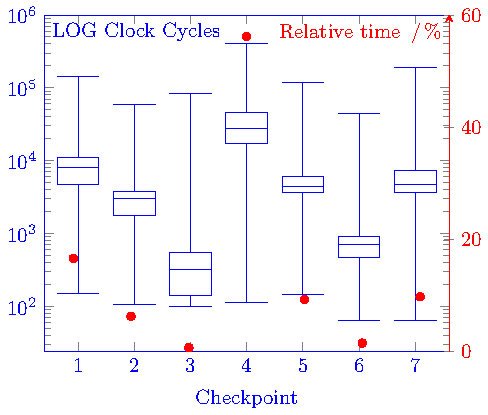
\includegraphics[width=0.8\columnwidth]{fig3cycles}
\caption{LOG Clock Cycles between checkpoints and relative time for each code segment\label{nosplitt}}
\end{figure}

\begin{figure}[htbp]\centering
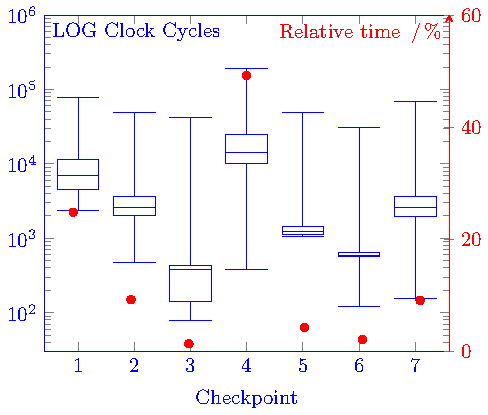
\includegraphics[width=0.8\columnwidth]{fig2cycles}
\caption{LOG Clock Cycles between checkpoints and relative time for each code segment, (shared splittings)\label{splitt}}
\end{figure}

\subsection{Experiment 2: GPU-CSG v/s DP}
Figure \ref{time} shows the difference between the CPU and GPU algorithms.
For every N agents the y axis shows the logarithmic elapsed time. The difference shown here between the implementations is substantial showing
that solving the problem on the GPU is highly beneficial. For 29 agents GPU-CSG employs 1.5 hours, while the CPU bound algorithm was extrapolated to show that it would take up to 83 hours to complete. This is a speedup factor of over 55, which is expected to grow with the number of agents. The reason it would grow is due to the implementations not being linearly parallel in logarithmic time where the GPU implementation having a smaller growth.

\begin{figure}[htbp]\centering
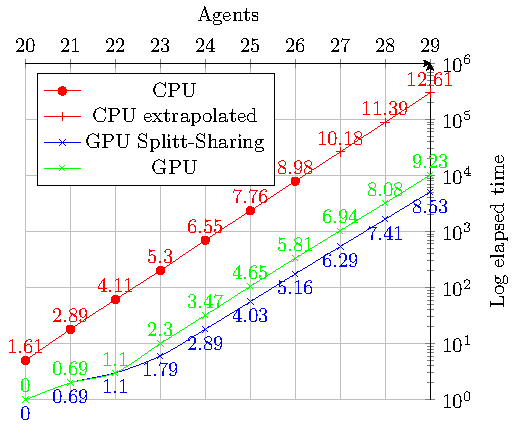
\includegraphics[width=0.8\columnwidth]{fig1cycles}
\caption{LOG elapsed time for N agents\label{time}}
\end{figure}
\section{Conclusion}
This paper presented the first GPU-based solution for the combinatorial optimisation problem of Coalition Structure Generation. Our algorithm, GPU-CSG, is shown to efficiently use memory access and thread allocation on the GPU in order to speed up the computations performed by a dynamic program for the CSG problem. In so doing, it is able to outperform the DP algorithm by up to 55 times, reducing the time taken to solve the problem for 29 agents to 1.5 hours as compared to 83 hours previously. Given the promising results of this initial work, we aim to develop new solutions for other similar optimisation problems in the future.

Further work would include incorporating the IDP technique and exploring further options to reduce memory bandwidth such as a more extensive collision detection.
At the moment of writing an algorithm implementing IDP and extensive collision detection have a speedup factor of 314 times at 28 agents.
\bibliographystyle{abbrv}
\bibliography{sigproc}  % sigproc.bib is the name of the Bibliography in this case
\end{document}
